\documentclass[a4paper]{article}
\usepackage{amsmath} % Define various maths environments
\usepackage{amssymb} % Define various maths symbols
\usepackage{geometry} % Adjust the margin, paper size, and etc.
\geometry{left=2.5cm,right=2.5cm,top=3cm,bottom=3cm}
\usepackage{enumerate} % Provide different style of lists
\usepackage{graphicx}
\usepackage{float}
\usepackage{listings} 

\title{—————————————————————————\\ \sc{UM-SJTU Joint Institute}}
\author{\sc{Data Structures and Algorithms}}
\date{\sc{(Ve281)}\\——————————————————————————————}

\begin{document}
\maketitle
\vspace{5cm}
\centerline{\Large{\sc{Lab 03 Report}}}
\vspace{9cm}
\begin{tabular}{lll}
\qquad \qquad Name: Sun Yiwen&ID: 517370910213\\
\qquad \qquad Date: 11 October 2019
\end{tabular}

\newpage
\section{Runtime Analysis}
\noindent
\par
I tested the five sorting algorithms with input array size $n=10,20,50,100,500,1000,10000$. The result is shown in Figure 1. In Figure 2, runtime of input size $n=10000$ is deleted in order to demonstrate the runtime difference between these five algorithms (when the input size is small) more clearly. As shown in these two plots, Bubble Sort and Insertion Sort have bigger runtimes while Merge Sort and Quick Sort have smaller runtimes. Selection Sort is something in between. This corresponds with the theoretical finding that Selection, Bubble and Insertion Sort have the average case time complexity of $O(n^2)$ while Merge and Quick Sort have the average case time complexity of $O(n\log n)$.

\begin{figure}[htbp]
\centering
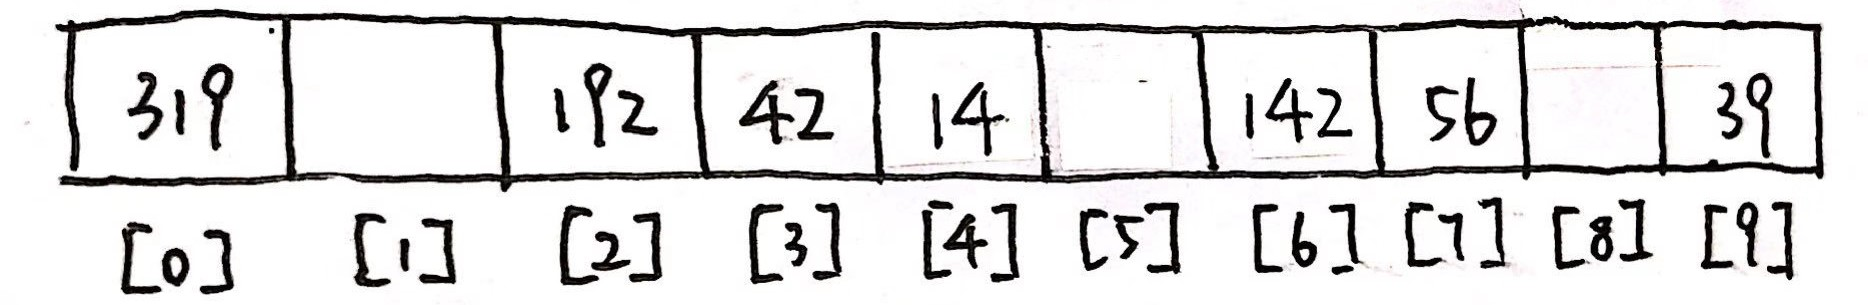
\includegraphics[scale=0.6]{f3.png}
\caption{Plot of runtime vs. array size of the five sorting algorithms. ($n_{max}=10000$)}
\end{figure}
\begin{figure}[htbp]
\centering
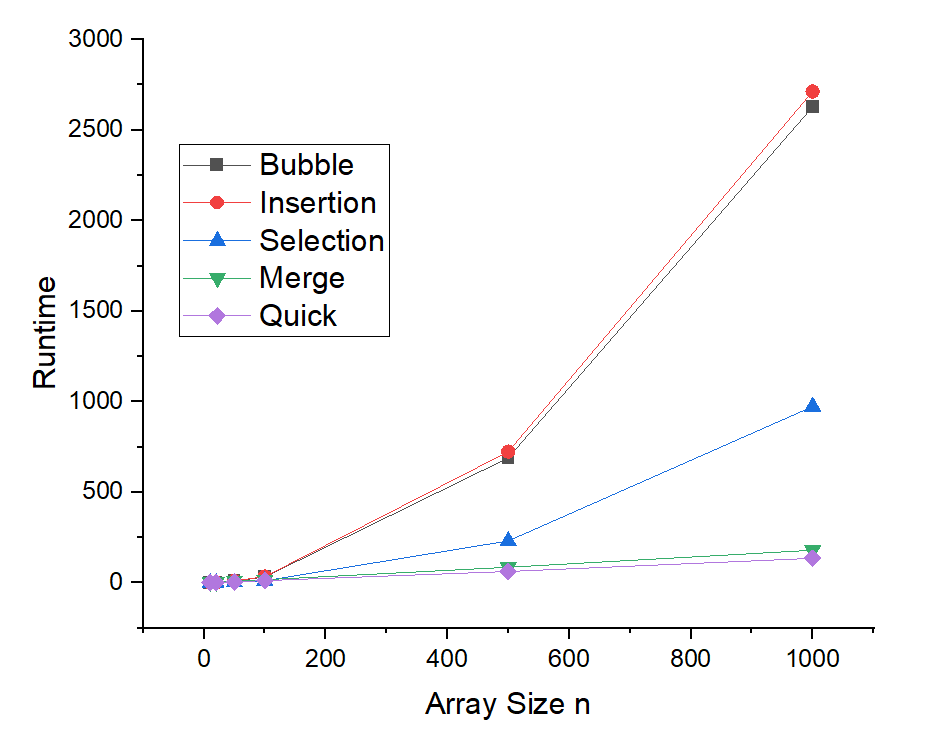
\includegraphics[scale=0.6]{f1.png}
\caption{Plot of runtime vs. array size of the five sorting algorithms. ($n_{max}=1000$)}
\end{figure}

\par
As shown in Figure 3 and Figure 4, I chose to test the algorithms using input size $n=10,20,50,100,500,1000,10000$. Quick Sort has the biggest runtime. Compared with Quick Sort, the linear time selection algorithms have smaller runtimes. Between these two, Random Selection has smaller run time than Deterministic Selection, which is very intriguing. Randomly choosing the pivot seems to work better than choosing the median of the medians as pivot. However, one thing good about Deterministic Selection is that its runtime is comparably more stable than Random Selection.


\begin{figure}[htbp]
\centering
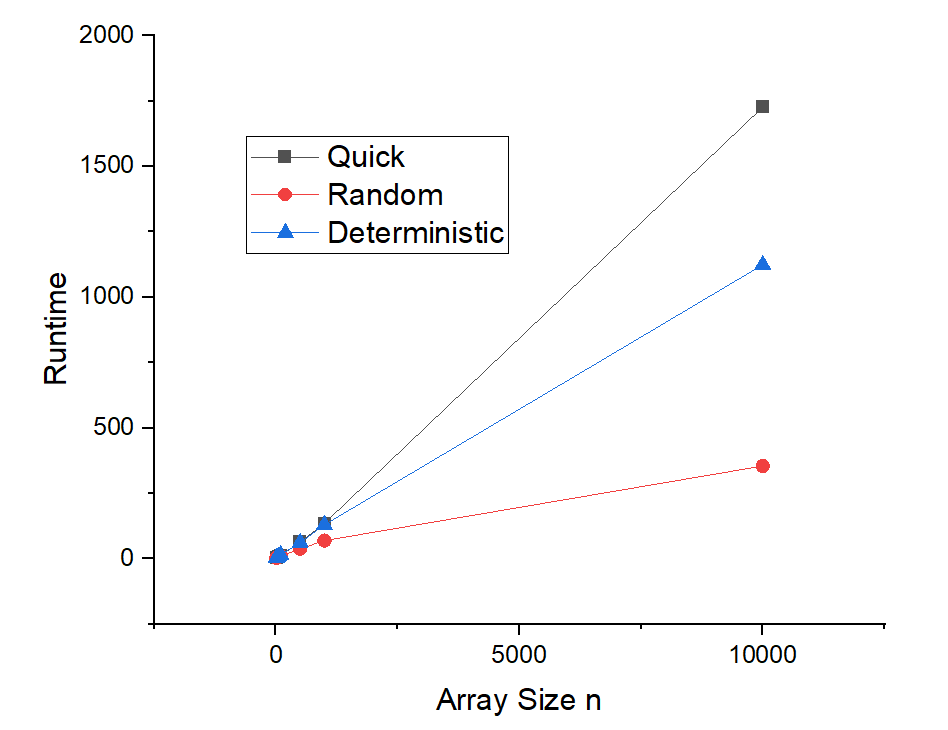
\includegraphics[scale=0.6]{f4.png}
\caption{Runtime vs. array size of Quick Sort, Random and Deterministic Selection. ($n_{max}=10000$)}
\end{figure}
\begin{figure}[htbp]
\centering
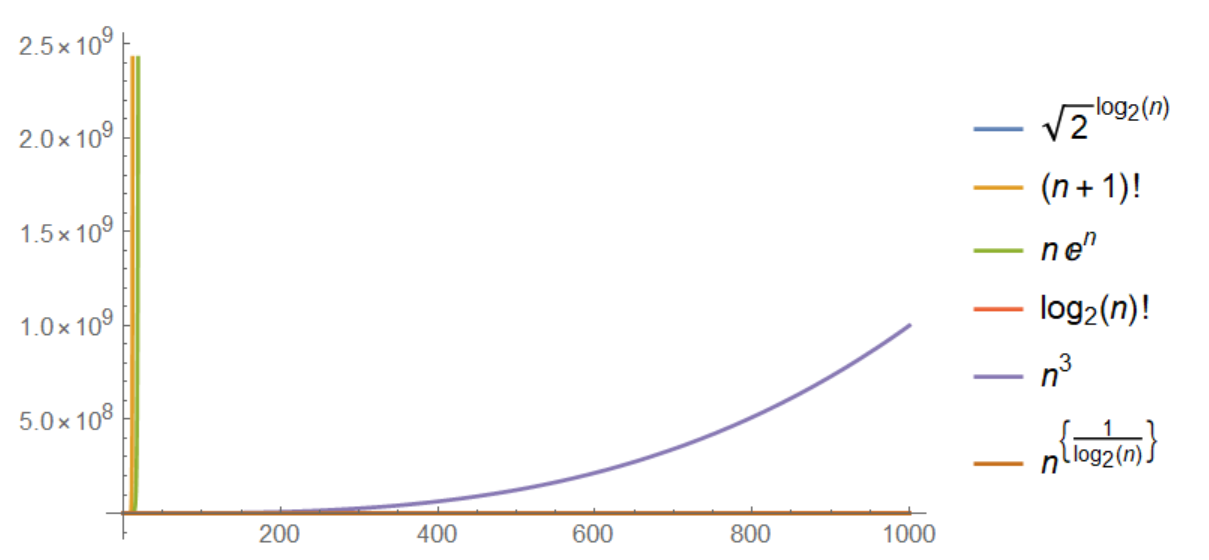
\includegraphics[scale=0.6]{f2.png}
\caption{Runtime vs. array size of Quick Sort, Random and Deterministic Selection. ($n_{max}=1000$)}
\end{figure}

\section{Code}
\begin{lstlisting}[language=C++] 
#include <iostream>
#include <fstream>
#include <sstream>
#include <string>
#include <cstdlib>
#include <climits>
#include <ctime>
#include <cassert>
using namespace std;

void bubbleSort(int a[], int n)
// MODIFIES: a[]
// EFFECTS: sort the array a[] in ascending order
{
	int i = 0;
	int j, temp;
	bool IsSorted = false;
	while (i < n && !IsSorted) {
		IsSorted = true;
		for (j = n - 1; j > i; j--) {
			if (a[j] < a[j - 1]) {
				temp = a[j];
				a[j] = a[j - 1];
				a[j - 1] = temp;
				IsSorted = false;
			}
		}
		i++;
	}
}

void selectionSort(int a[], int n)
// MODIFIES: a[]
// EFFECTS: sort the array a[] in ascending order
{
	int i, j, temp;
	for (i = 0; i < n; i++) {
		for (j = i + 1; j < n; j++) {
			if (a[i] > a[j]) {
				temp = a[i];
				a[i] = a[j];
				a[j] = temp;
			}
		}
	}
}

void insertionSort(int a[], int n)
// MODIFIES: a[]
// EFFECTS: sort the array a[] in ascending order
{
	int i, j, temp;
	for (i = 1; i < n; i++) {
		temp = a[i];
		j = i - 1;
		while (j >= 0 && a[j] > temp) {
			a[j + 1] = a[j];
			j = j - 1;
		}
		a[j + 1] = temp;
	}
}

void merge(int a[], int left, int mid, int right)
// MODIFIES: a[]
// EFFECTS: sort the array a[] in ascending order
{
	int i = left;
	int j = mid + 1;
	int k = 0;
	int* temp = new int[right - left + 1];
	while (i <= mid && j <= right) {
		if (a[i] <= a[j]) temp[k++] = a[i++];
		else temp[k++] = a[j++];
	}
	if (i == mid + 1) {
		while (j <= right) {
			temp[k++] = a[j++];
		}
	}
	else {
		while (i <= mid) {
			temp[k++] = a[i++];
		}
	}
	i = 0;
	for (j = left; j <= right; j++) a[j] = temp[i++];
	delete[] temp;
}

void mergeSort(int a[], int left, int right)
// MODIFIES: a[]
// EFFECTS: sort the array a[] in ascending order
{
	int mid;
	if (left >= right) {
		return;
	}
	mid = (left + right) / 2;
	mergeSort(a, left, mid);
	mergeSort(a, mid + 1, right);
	merge(a, left, mid, right);
}

void quickSort(int a[], int left, int right)
// MODIFIES: a[]
// EFFECTS: sort the array a[] in ascending order
{
	int i = left + 1, j = right, pivotat, pivot, temp;
	bool partition = true;
	pivotat = left + rand() % (right - left + 1);
	pivot = a[pivotat];
	temp = a[left];
	a[left] = pivot;
	a[pivotat] = temp;
	while (partition) {
		while (i < right && a[i] < pivot) i++;
		while (j > left && a[j] >= pivot) j--;
		if (i < j) {
			temp = a[i];
			a[i] = a[j];
			a[j] = temp;
		}
		else {
			temp = a[left];
			a[left] = a[j];
			a[j] = temp;
			partition = false;
		}
	}
	if (left < j - 1) quickSort(a, left, j - 1);
	if (j + 1 < right) quickSort(a, j + 1, right);
}

int randomSel(int a[], int n, int i)
// EFFECTS: return the i-th smallest item in the array a[]
{
	int m = 0, j = 0, k = n - 1, pivot, pivotat, res;
	int* temp = new int[n];
	if (n == 1) return a[0];
// choosing the pivot randomly
	pivotat = rand() % n;
	pivot = a[pivotat];
	while (m < n) {
		if (a[m] < pivot && m != pivotat) temp[j++] = a[m++];
		else if (a[m] >= pivot && m != pivotat) temp[k--] = a[m++];
		else m++;
	}
	temp[j] = pivot;
	for (m = 0; m < n; m++) a[m] = temp[m];
	delete[] temp;
	if (j == i) return pivot;
	if (j > i) {
		int* a1 = new int[j];
		for (m = 0; m < j; m++) {
			a1[m] = a[m];
		}
		res = randomSel(a1, j, i);
		delete[] a1;
		return res;
	}
	else {
		int* a2 = new int[n - j - 1];
		for (m = 0; m < n - j - 1; m++) {
			a2[m] = a[m + j + 1];
		}
		res = randomSel(a2, n - j - 1, i - j - 1);
		delete[] a2;
		return res;
	}
}

int deterministicSel(int a[], int n, int i)
// EFFECTS: return the i-th smallest item in the array a[]
{
	int m, p, j = 0, k = n - 1, pivot, pivotat = 0, res, n_new, n_mod, t[5];
	if (n == 1) return a[0];
// choosing the median of medians as pivot
	n_mod = n % 5;
	if (n_mod == 0) n_new = n / 5;
	else n_new = n / 5 + 1;
	int* b = new int[n_new];
	for (m = 0; m < n / 5 * 5; m = m + 5) {
		p = 0;
		while (p < 5 && p < n) {
			t[p] = a[m + p];
			p++;
		}
		insertionSort(t, 5);
		b[m / 5] = t[2];
	}
	int* c = new int[n_mod];
	for (p = 0; p < n_mod; p++) {
		c[p] = a[n / 5 * 5 + p];
	}
	insertionSort(c, n_mod);
	if (n_mod != 0) b[n_new - 1] = c[n_mod / 2];
	delete[] c;
	if (n_new == 1) pivot = b[0];
	else pivot = deterministicSel(b, n / 5, n / 10);
	delete[] b;
	for (m = 0; m < n; m++) {
		if (a[m] == pivot) {
			pivotat = m;
			break;
		}
	}
// the rest is same as Random Selection
	m = 0;
	int* temp = new int[n];
	while (m < n) {
		if (a[m] < pivot && m != pivotat) temp[j++] = a[m++];
		else if (a[m] >= pivot && m != pivotat) temp[k--] = a[m++];
		else m++;
	}
	temp[j] = pivot;
	pivotat = j;
	for (m = 0; m < n; m++) a[m] = temp[m];
	delete[] temp;
	if (j == i) return pivot;
	if (j > i) {
		int* a1 = new int[j];
		for (m = 0; m < j; m++) {
			a1[m] = a[m];
		}
		res = deterministicSel(a1, j, i);
		delete[] a1;
		return res;
	}
	else {
		int* a2 = new int[n - j - 1];
		for (m = 0; m < n - j - 1; m++) {
			a2[m] = a[m + j + 1];
		}
		res = deterministicSel(a2, n - j - 1, i - j - 1);
		delete[] a2;
		return res;
	}
}

int main() {
	int type, n, i, m, res = 0;
	cin >> type >> n;
	int* a = new int[n];
	if (type > 4) {
		cin >> i;
	}
	for (m = 0; m < n; m++) {
		cin >> a[m];
	}
	switch (type)
	{
		case 0:
			bubbleSort(a, n);
			break;
		case 1:
			selectionSort(a, n);
			break;
		case 2:
			insertionSort(a, n);
			break;
		case 3:
			mergeSort(a, 0, n - 1);
			break;
		case 4:
			quickSort(a, 0, n - 1);
			break;
		case 5:
			res = randomSel(a, n, i);
			break;
		case 6:
			res = deterministicSel(a, n, i);
			break;
	}
	if (type < 5) {
		for (m = 0; m < n; m++) {
			cout << a[m] << endl;
		}
	}
	else cout << "The order-" << i << " item is " << res << endl;
	delete[] a;
	return 0;
}
\end{lstlisting}


\end{document}